\documentclass[a4paper, final]{article}
\usepackage[14pt]{extsizes} % для того чтобы задать нестандартный 14-ый размер шрифта
\usepackage[T2A]{fontenc}
\usepackage[utf8]{inputenc}
\usepackage[russian]{babel}
\usepackage{ragged2e}
\usepackage{tabularx}
\usepackage{array}
\usepackage{amsmath}
\usepackage{multirow}
\usepackage{multicol}
\usepackage{stackrel}
\usepackage[left=25mm, top=20mm, right=20mm, bottom=20mm, footskip=10mm]{geometry}
\usepackage{ragged2e} %для растягивания по ширине
\usepackage{setspace} %для межстрочного интервала
\usepackage{moreverb} %для работы с листингами
\usepackage{indentfirst} % для абзацного отступа
\usepackage{moreverb} %для печати в листинге исходного кода программ
\renewcommand\verbatimtabsize{4\relax}
\renewcommand\listingoffset{0.2em}
\renewcommand{\arraystretch}{1.4} % изменяю высоту строки в таблице
\usepackage[font=small, singlelinecheck=false, justification=raggedleft, format=plain, labelsep=period]{caption} %для настройки заголовка таблицы
\usepackage[dvips]{graphicx} % Для вставки графических изображений
\graphicspath{{noiseimages/}}
\usepackage{color} %% это для отображения цвета в коде
\usepackage{xcolor} % цвета
\usepackage{listingsutf8}
\usepackage{hyperref}% для гиперссылок
\usepackage{enumitem} %для перечислений
\usepackage{pdflscape} %для pdf
\usepackage{pdfpages} %для pdf

\definecolor{apricot}{HTML}{FFF0DA}
\definecolor{mygreen}{rgb}{0,0.6,0}
\definecolor{string}{HTML}{B40000} % цвет строк в коде
\definecolor{comment}{HTML}{008000} % цвет комментариев в коде
\definecolor{keyword}{HTML}{1A00FF} % цвет ключевых слов в коде
\definecolor{morecomment}{HTML}{8000FF} % цвет include и других элементов в коде
\definecolor{captiontext}{HTML}{FFFFFF} % цвет текста заголовка в коде
\definecolor{captionbk}{HTML}{999999} % цвет фона заголовка в коде
\definecolor{bk}{HTML}{FFFFFF} % цвет фона в коде
\definecolor{frame}{HTML}{999999} % цвет рамки в коде
\definecolor{brackets}{HTML}{B40000} % цвет скобок в коде

\setlist[enumerate,itemize]{leftmargin=1.2cm}

\hypersetup{colorlinks,
	pdftitle={Отчёт по второй лабе Лобанов},
	pdfauthor={Your name},
	allcolors=[RGB]{010 090 200}}
% подгружаемые языки — подробнее в документации listings
\lstloadlanguages{Java}
% включаем кириллицу и добавляем кое−какие опции
%\lstset{language =[LaTeX] TeX, % выбираем язык по умолчанию
	%extendedchars=true , % включаем не латиницу
	%escapechar = | , % |«выпадаем» в LATEX|
	%frame=tb , % рамка сверху и снизу
	%commentstyle=\itshape , % шрифт для комментариев
	%stringstyle =\bfseries} % шрифт для строк

\textheight=24cm % высота текста
\textwidth=16cm % ширина текста
\oddsidemargin=0pt % отступ от левого края
\topmargin=-1.5cm % отступ от верхнего края
\parindent=24pt % абзацный отступ
\parskip=0pt % интервал между абзацами
\tolerance=2000 % терпимость к "жидким" строкам
\flushbottom % выравнивание высоты страниц

\addto\captionsrussian{\def\refname{\hspace{1.15cm} Список литературы}}

\begin{document} % начало документа
	
	\lstset{
		language=Java, % Язык кода по умолчанию
		morekeywords={*,...}, % если хотите добавить ключевые слова, то добавляйте
		% Цвета
		keywordstyle=\color{keyword}\ttfamily\bfseries,
		%stringstyle=\color{string}\ttfamily,
		stringstyle=\ttfamily\color{red!50!brown},
		commentstyle=\color{comment}\ttfamily,
		morecomment=[l][\color{morecomment}]{\#},
		% Настройки отображения
		breaklines=true, % Перенос длинных строк
		basicstyle=\ttfamily\footnotesize, % Шрифт для отображения кода
		backgroundcolor=\color{bk}, % Цвет фона кода
		frame=lrb,xleftmargin=\fboxsep,xrightmargin=-\fboxsep, % Рамка, подогнанная к заголовку
		rulecolor=\color{frame}, % Цвет рамки
		tabsize=3, % Размер табуляции в пробелах
		% Настройка отображения номеров строк. Если не нужно, то удалите весь блок
		numbers=left, % Слева отображаются номера строк
		stepnumber=1, % Каждую строку нумеровать
		numbersep=5pt, % Отступ от кода
		numberstyle=\small\color{black}, % Стиль написания номеров строк
		% Для отображения русского языка
		extendedchars=true,
		literate={Ö}{ {\"O} }1
		{~}{ {\textasciitilde} }1
		{а}{ {\selectfont\char224} }1
		{б}{ {\selectfont\char225} }1
		{в}{ {\selectfont\char226} }1
		{г}{ {\selectfont\char227} }1
		{д}{ {\selectfont\char228} }1
		{е}{ {\selectfont\char229} }1
		{ё}{ {\"e} }1
		{ж}{ {\selectfont\char230} }1
		{з}{ {\selectfont\char231} }1
		{и}{ {\selectfont\char232} }1
		{й}{ {\selectfont\char233} }1
		{к}{ {\selectfont\char234} }1
		{л}{ {\selectfont\char235} }1
		{м}{ {\selectfont\char236} }1
		{н}{ {\selectfont\char237} }1
		{о}{ {\selectfont\char238} }1
		{п}{ {\selectfont\char239} }1
		{р}{ {\selectfont\char240} }1
		{с}{ {\selectfont\char241} }1
		{т}{ {\selectfont\char242} }1
		{у}{ {\selectfont\char243} }1
		{ф}{ {\selectfont\char244} }1
		{х}{ {\selectfont\char245} }1
		{ц}{ {\selectfont\char246} }1
		{ч}{ {\selectfont\char247} }1
		{ш}{ {\selectfont\char248} }1
		{щ}{ {\selectfont\char249} }1
		{ъ}{ {\selectfont\char250} }1
		{ы}{ {\selectfont\char251} }1
		{ь}{ {\selectfont\char252} }1
		{э}{ {\selectfont\char253} }1
		{ю}{ {\selectfont\char254} }1
		{я}{ {\selectfont\char255} }1
		{А}{ {\selectfont\char192} }1
		{Б}{ {\selectfont\char193} }1
		{В}{ {\selectfont\char194} }1
		{Г}{ {\selectfont\char195} }1
		{Д}{ {\selectfont\char196} }1
		{Е}{ {\selectfont\char197} }1
		{Ё}{ {\"E} }1
		{Ж}{ {\selectfont\char198} }1
		{З}{ {\selectfont\char199} }1
		{И}{ {\selectfont\char200} }1
		{Й}{ {\selectfont\char201} }1
		{К}{ {\selectfont\char202} }1
		{Л}{ {\selectfont\char203} }1
		{М}{ {\selectfont\char204} }1
		{Н}{ {\selectfont\char205} }1
		{О}{ {\selectfont\char206} }1
		{П}{ {\selectfont\char207} }1
		{Р}{ {\selectfont\char208} }1
		{С}{ {\selectfont\char209} }1
		{Т}{ {\selectfont\char210} }1
		{У}{ {\selectfont\char211} }1
		{Ф}{ {\selectfont\char212} }1
		{Х}{ {\selectfont\char213} }1
		{Ц}{ {\selectfont\char214} }1
		{Ч}{ {\selectfont\char215} }1
		{Ш}{ {\selectfont\char216} }1
		{Щ}{ {\selectfont\char217} }1
		{Ъ}{ {\selectfont\char218} }1
		{Ы}{ {\selectfont\char219} }1
		{Ь}{ {\selectfont\char220} }1
		{Э}{ {\selectfont\char221} }1
		{Ю}{ {\selectfont\char222} }1
		{Я}{ {\selectfont\char223} }1
		{\{}{ { {\color{brackets}\{} } }1 % Цвет скобок {
			{\} }{ { {\color{brackets}\} } } }1 % Цвет скобок }
	}
	
	
	% НАЧАЛО ТИТУЛЬНОГО ЛИСТА
	\thispagestyle{empty}
	\begin{center}
		\normalsize{МИНИСТЕРСТВО НАУКИ И ВЫСШЕГО ОБРАЗОВАНИЯ РОССИЙСКОЙ ФЕДЕРАЦИИ \\ ФЕДЕРАЛЬНОЕ ГОСУДАРСТВЕННОЕ АВТОНОМНОЕ ОБРАЗОВАТЕЛЬНОЕ УЧРЕЖДЕНИЕ ВЫСШЕГО \\ ОБРАЗОВАНИЯ\\ «Санкт-Петербургский политехнический университет Петра Великого»}
		\normalsize{Институт компьютерных наук и кибербезопастности}\\[3pt]
		\normalsize{Высшая школа технологий искусственного интеллекта}\\[10pt]
		\normalsize{Направление: 02.04.01 Математика и компьютерные науки}\\[10pt]
		\hfill \break
		\hfill \break
		\hfill \break
		\hfill \break
		\hfill \break
		\hfill \break
		\normalsize{Отчет по ИДЗ №2:}\\
		\normalsize{по дисциплине «Элементы теории вероятности и линейной алгебры»}\\
		\normalsize{Вариант №12}\\[10pt]
	\end{center}
	\hfill \break
	\hfill \break
	\hfill \break
	\hfill \break
	\begin{tabular}{lcrl}	
		\!\!\!Студент, & \hspace{2cm} & & \\
		\!\!\!группы 5140201/60301 & \hspace{2.13cm} & \underline{\hspace{3cm}} &Лобанов П. М. \\\\
		\!\!\!Преподаватель & \hspace{2cm}  & \underline{\hspace{3cm}} &\hspace{0pt} Малов С. В. \\\\	
		&&\hspace{5cm}
		
	\end{tabular} 	
	\begin{flushright}
		<<\underline{\hspace{1cm}}>>\underline{\hspace{2.5cm}} 2026 г.
	\end{flushright}
	\hfill \break
	\hfill \break
	\hfill \break
	\begin{center} \small{Санкт-Петербург, 2026} \end{center}
	\newpage %Содержание% выключаем отображение номера для этой страницы
	
	
	\section*{Задание}
	
	\begin{figure}[h!]
		\centering
		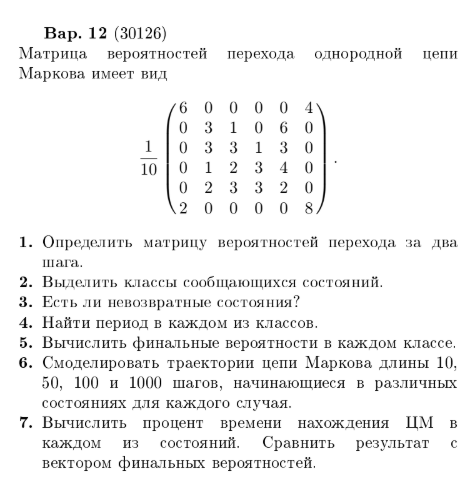
\includegraphics[width=110mm]{task}
		\caption{\centering{Задание для варианта 12}}
		\label{fig:task}
	\end{figure}
	
	\subsection*{Задание 1. Матрица вероятностей перехода за два шага}
	
	Для однородной цепи Маркова матрица переходных
	вероятностей за $n$ шагов определяется как
	\[
	P^{(n)}=P^n.
	\]
	
	Следовательно, матрица переходов за два шага равна
	произведению исходной матрицы на саму себя:
	\[
	P^{(2)}=P\cdot P.
	\]
	
	Каждый элемент полученной матрицы вычисляется по формуле
	\[
	p_{ij}^{(2)}=\sum_{k=1}^{6}p_{ik}p_{kj}.
	\]
	
	В результате получаем матрицу:
	
	\[
		P^{(2)}=\frac{1}{100}
		\begin{pmatrix}
			44&0&0&0&0&56\\
			0&24&24&19&33&0\\
			0&25&23&15&37&0\\
			0&20&25&23&32&0\\
			0&22&23&18&37&0\\
			28&0&0&0&0&72
		\end{pmatrix}
	\]
	
	Для проверки результата вычислим сумму элементов
	каждой строки:
	
	\[
	\begin{aligned}
		&\frac{44+56}{100}=1,\\
		&\frac{24+24+19+33}{100}=1,\\
		&\frac{25+23+15+37}{100}=1,\\
		&\frac{20+25+23+32}{100}=1,\\
		&\frac{22+23+18+37}{100}=1,\\
		&\frac{28+72}{100}=1.
	\end{aligned}
	\]
	
	Все строки полученной матрицы имеют сумму 1.
	Следовательно, матрица $P^{(2)}$ также является
	стохастической.
	
	\subsection*{Задание 2. Классы сообщающихся состояний}
	
	Состояния $i$ и $j$ называются сообщающимися,
	если существует путь из состояния $i$ в $j$ и
	обратный путь из $j$ в $i$:
	\[
	i\leftrightarrow j.
	\]
	
	По структуре исходной матрицы переходов можно
	выделить две группы состояний.
	
	Для первой группы выполняется:
	\[
	v_1\leftrightarrow v_6,
	\]
	поскольку существуют переходы
	\[
	v_1\rightarrow v_6,\qquad
	v_6\rightarrow v_1.
	\]
	
	Следовательно, первый класс сообщающихся состояний:
	\[
	K_1=\{v_1,v_6\}.
	\]
	
	Для второй группы состояний проверим взаимную
	достижимость:
	
	\[
	\begin{aligned}
		v_2\leftrightarrow v_3 &:\
		v_2\rightarrow v_3,\quad v_3\rightarrow v_2;\\
		v_2\leftrightarrow v_4 &:\
		v_2\rightarrow v_3\rightarrow v_4,\quad
		v_4\rightarrow v_2;\\
		v_2\leftrightarrow v_5 &:\
		v_2\rightarrow v_5,\quad v_5\rightarrow v_2;\\
		v_3\leftrightarrow v_4 &:\
		v_3\rightarrow v_4,\quad v_4\rightarrow v_3;\\
		v_3\leftrightarrow v_5 &:\
		v_3\rightarrow v_5,\quad v_5\rightarrow v_3;\\
		v_4\leftrightarrow v_5 &:\
		v_4\rightarrow v_5,\quad v_5\rightarrow v_4.
	\end{aligned}
	\]
	
	Таким образом, второй класс:
	\[
	K_2=\{v_2,v_3,v_4,v_5\}.
	\]
	
	\subsection*{Задание 3. Невозвратные состояния}
	
Внутри двух сообщающихся классов все состояния являются взаимно сообщаемыми с каждым состоянием в классе, значит нет такого случая, чтобы из любого состояния нельзя было бы вернуться в самого себя. А значит все состояния — возвратные.
	
	\subsection*{Задание 4. Периоды классов}
	
	Период состояния $i$ определяется как наибольший
	общий делитель всех возможных времен возвращения
	в данное состояние:
	$	T_i=\operatorname{НОД}
	\{n\geq 1:p_{ii}^{(n)}>0\}$
	
	Все состояния одного класса сообщающихся
	состояний имеют одинаковый период.
	
	Рассмотрим первый класс:
$
	K_1=\{v_1,v_6\}.
$
	Внутри класса возможны переходы в самих себя. Следовательно НОД с любом случае = 1.
	
	Рассмотрим второй класс:
$
	K_2=\{v_2,v_3,v_4,v_5\}.
$
	
	Все состояния этого класса имеют положительные
	вероятности перехода в самих себя, таким образом, аналогично первому классу возврат в каждое состояние
	возможен за один шаг. Следовательно,
	\[
	{T_{K_2}=1}
	\]
	
	Оба класса имеют период 1 и являются
	непериодическими.
	
	\subsection*{Задание 5. Вычисление финальных вероятностей}
	\subsubsection*{Первый класс}
	Матрица переходов класса $
	K_1=\{v_1,v_6\} 
	$имеет вид

	\[
	P_{K_1}=\frac1{10}
	\begin{pmatrix}
		6&4\\
		2&8
	\end{pmatrix}.
	\]
	
	Обозначим вектор финальных вероятностей:
	\[
	\pi^{(1)}=(\pi_1,\pi_6).
	\]
	
	Из условия $\pi^{(1)}P_{K_1}=\pi^{(1)}$
	получаем систему:
	\[
	\begin{cases}
		10\pi_1=6\pi_1+2\pi_6,\\
		10\pi_6=4\pi_1+8\pi_6,\\
		\pi_1+\pi_6=1.
	\end{cases}
	\]
	
	\[
	\begin{aligned}
		\begin{cases}
			10\pi_1=6\pi_1+2\pi_6,\\
			10\pi_6=4\pi_1+8\pi_6,\\
			\pi_1+\pi_6=1.
		\end{cases}
		&\Rightarrow\qquad
		\begin{cases}
			4\pi_1=2\pi_6,\\
			2\pi_6=4\pi_1,\\
			\pi_1+\pi_6=1.
		\end{cases}
	\end{aligned}
	\]
Из третьего уравнения получаем:
	$
	\begin{aligned}
		\pi_1&=\frac13.
	\end{aligned}
$	Тогда:
$\displaystyle
\pi_6=2\cdot\frac13=\frac23.
$ 
	


	Следовательно, вектор финальных вероятностей
	первого класса:
	\[
	{
		\pi^{(1)}=\left(\frac13,\frac23\right)
	}
	\]
	
	\subsubsection*{Второй класс}
	
	Матрица переходов класса $ K_2=\{v_2,v_3,v_4,v_5\}$ имеет вид:
	\[
	P_{K_2}=\frac1{10}
	\begin{pmatrix}
		3&1&0&6\\
		3&3&1&3\\
		1&2&3&4\\
		2&3&3&2
	\end{pmatrix}.
	\]
	
	Вектор финальных вероятностей:
	\[
	\pi^{(2)}=(\pi_2,\pi_3,\pi_4,\pi_5).
	\]
	
	Из условия $\pi^{(2)}P_{K_2}=\pi^{(2)}$
	получаем следующую систему:
	\[
	\begin{aligned}
	\begin{cases}
		10\pi_2=3\pi_2+3\pi_3+\pi_4+2\pi_5,\\
		10\pi_3=\pi_2+3\pi_3+2\pi_4+3\pi_5,\\
		10\pi_4=\pi_3+3\pi_4+3\pi_5,\\
		10\pi_5=6\pi_2+3\pi_3+4\pi_4+2\pi_5,\\
		\pi_2+\pi_3+\pi_4+\pi_5=1.
	\end{cases}
	&\Rightarrow
		\begin{cases}
		7\pi_2-3\pi_3-\pi_4-2\pi_5=0,\\
		-\pi_2+7\pi_3-2\pi_4-3\pi_5=0,\\
		-\pi_3+7\pi_4-3\pi_5=0,\\
		-6\pi_2-3\pi_3-4\pi_4+8\pi_5=0,\\
		\pi_2+\pi_3+\pi_4+\pi_5=1.
	\end{cases}
	\end{aligned}
	\]
	
	Из третьего уравнения:
	\[
	{\pi_3=7\pi_4-3\pi_5}
	\]
	
	Подставим данное выражение в первое уравнение:
	\[
	7\pi_2-3(7\pi_4-3\pi_5)-\pi_4-2\pi_5=0.
	\]
	
	После раскрытия скобок:
	\[
	7\pi_2-22\pi_4+7\pi_5=0.
	\]
	
	Следовательно:
	\[
	{
		\pi_2=\frac{22}{7}\pi_4-\pi_5
	}.
	\]
	
	Подставим полученные выражения для $\pi_2$
	и $\pi_3$ во второе уравнение:
	\[
	-\left(\frac{22}{7}\pi_4-\pi_5\right)
	+7(7\pi_4-3\pi_5)
	-2\pi_4-3\pi_5=0.
	\]
	
	
	Отсюда:
	\[
	{
		\pi_4=\frac{161}{307}\pi_5
	}.
	\]
	
	Выразим оставшиеся вероятности через $\pi_5$:
	\[
	\begin{aligned}
		\pi_3
		&=7\cdot\frac{161}{307}\pi_5-3\pi_5
		=\frac{206}{307}\pi_5,\\
		\pi_2
		&=\frac{22}{7}\cdot\frac{161}{307}\pi_5-\pi_5
		=\frac{199}{307}\pi_5.
	\end{aligned}
	\]
	
	Используем условие нормировки:
	\[
	\pi_2+\pi_3+\pi_4+\pi_5=1.
	\]
	
	Подставим найденные выражения:
	\[
	\frac{199}{307}\pi_5+
	\frac{206}{307}\pi_5+
	\frac{161}{307}\pi_5+
	\pi_5=1.
	\]
	
	Получаем:
	\[
	\frac{873}{307}\pi_5=1,
	\qquad
	\pi_5=\frac{307}{873}.
	\]
	
	Следовательно:
	\[
	\begin{aligned}
		\pi_2&=\frac{199}{873},\\
		\pi_3&=\frac{206}{873},\\
		\pi_4&=\frac{161}{873},\\
		\pi_5&=\frac{307}{873}.
	\end{aligned}
	\]
	
	Вектор финальных вероятностей второго класса:
	\[
	{
		\pi^{(2)}=
		\left(
		\frac{199}{873},
		\frac{206}{873},
		\frac{161}{873},
		\frac{307}{873}
		\right)
	}.
	\]
	
	
	Проверим условия нормировки:
	\[
	\frac13+\frac23=1,
	\]
	\[
	\frac{199+206+161+307}{873}=1.
	\]
	
\subsection*{Задание 6. Моделирование траекторий}
Переход выбирается случайно по строке $P$ для текущего состояния.
Моделирование выполнено из каждого из шести состояний на
10, 50, 100 и 1000 шагов (24 траектории).
\lstset{
	frame= single}
\begin{lstlisting}[language=Python]
class MarkovChain:
	def __init__(self, transition_matrix):
		self.transition_matrix = transition_matrix
	
	def step(self, state):
		return int(np.random.choice(
		len(self.transition_matrix),
		p=self.transition_matrix[state]))
	
	def simulate(self, start_state, num_steps):
		states = [start_state]
		current_state = start_state
		for _ in range(num_steps):
			current_state = self.step(current_state)
			states.append(current_state)
		return states

markov_chain = MarkovChain(P)
result_map = {}
for start_state in range(len(P)):
	for n in [10, 50, 100, 1000]:
		result_map[(start_state, n)] = (
		markov_chain.simulate(start_state, n))
\end{lstlisting}
Ниже приведены переходы для 10, 50, 100 и 1000 переходов. Первое число в списке - первое состояние после первого перехода.

\subsubsection*{Последовательности переходов}
\begingroup
\fontsize{7}{8}\selectfont
\setlength{\columnsep}{11pt}
\begin{multicols}{2}
	\raggedright
	\noindent\textbf{Начальное состояние $v_1$}\par
	\noindent\textbf{10 шагов:}6, 6, 6, 1, 6, 6, 1, 6, 6, 6\par\smallskip
	\medskip
	\noindent\textbf{Начальное состояние $v_2$}\par
	\noindent\textbf{50 шагов:} 5, 4, 4, 5, 2, 5, 4, 3, 2, 5, 4, 5, 2, 5, 5, 2, 2, 5, 4, 5, 4, 4, 4, 5, 4, 4, 4, 5, 2, 2, 2, 5, 4, 5, 2, 2, 5, 4, 5, 4, 5, 3, 3, 3, 5, 5, 5, 4, 5, 3\par\smallskip
	\medskip
	\noindent\textbf{Начальное состояние $v_3$}\par
	\noindent\textbf{100 шагов:}  5, 4, 3, 2, 2, 5, 4, 3, 3, 3, 5, 4, 2, 5, 2, 2, 2, 2, 2, 5, 2, 5, 2, 5, 4, 4, 4, 2, 2, 2, 3, 2, 5, 5, 5, 4, 5, 4, 5, 3, 2, 5, 4, 5, 3, 3, 4, 4, 5, 3, 4, 5, 2, 5, 2, 5, 3, 3, 3, 3, 4, 5, 3, 5, 2, 2, 2, 2, 5, 4, 3, 4, 5, 3, 3, 5, 3, 5, 2, 5, 4, 4, 4, 2, 5, 4, 4, 5, 2, 2, 5, 5, 4, 3, 2, 5, 2, 2, 3, 2\par\smallskip
	\medskip
	\noindent\textbf{Начальное состояние $v_5$}\par
	\noindent\textbf{1000 шагов:} 2, 5, 4, 4, 4, 3, 3, 2, 5, 2, 3, 3, 2, 5, 3, 5, 2, 2, 5, 3, 2, 5, 2, 5, 5, 3, 2, 5, 5, 4, 4, 4, 5, 5, 4, 3, 5, 2, 5, 5, 5, 4, 5, 4, 2, 5, 5, 4, 4, 4, 4, 5, 4, 5, 3, 3, 5, 3, 5, 3, 3, 2, 2, 2, 5, 5, 2, 5, 4, 4, 3, 3, 2, 2, 2, 5, 3, 2, 5, 3, 5, 2, 3, 5, 5, 4, 5, 5, 5, 3, 2, 5, 2, 5, 4, 2, 5, 5, 2, 5, 3, 5, 3, 4, 4, 4, 4, 2, 5, 2, 2, 5, 2, 5, 4, 3, 4, 2, 5, 2, 2, 3, 2, 5, 4, 4, 5, 2, 2, 5, 3, 2, 5, 4, 4, 3, 3, 4, 3, 2, 5, 3, 3, 4, 4, 4, 4, 5, 3, 3, 3, 3, 2, 3, 5, 3, 5, 2, 3, 3, 3, 2, 2, 5, 2, 2, 2, 3, 3, 5, 5, 3, 5, 4, 3, 2, 5, 2, 3, 3, 5, 3, 3, 3, 5, 2, 2, 5, 5, 3, 2, 3, 5, 5, 4, 5, 2, 2, 5, 3, 3, 2, 2, 2, 5, 3, 5, 5, 4, 3, 5, 4, 3, 3, 4, 5, 5, 4, 5, 4, 5, 4, 4, 3, 5, 3, 3, 3, 2, 5, 2, 2, 5, 5, 4, 3, 5, 4, 4, 5, 3, 3, 5, 2, 2, 5, 4, 4, 5, 4, 5, 3, 5, 3, 3, 2, 5, 4, 3, 4, 5, 3, 5, 2, 5, 4, 4, 4, 4, 5, 5, 5, 2, 3, 5, 2, 5, 3, 2, 5, 4, 3, 3, 2, 5, 3, 5, 4, 5, 4, 4, 4, 3, 3, 5, 5, 3, 2, 5, 2, 5, 4, 4, 5, 4, 5, 3, 4, 4, 4, 4, 5, 5, 5, 3, 3, 3, 3, 5, 5, 5, 5, 5, 2, 5, 2, 5, 5, 4, 5, 5, 5, 2, 2, 3, 2, 5, 4, 4, 5, 2, 5, 3, 4, 5, 2, 3, 3, 3, 5, 3, 3, 4, 4, 4, 4, 5, 2, 3, 2, 3, 3, 3, 2, 5, 4, 4, 4, 3, 2, 3, 5, 4, 5, 2, 5, 3, 2, 2, 5, 3, 2, 5, 2, 5, 2, 5, 5, 3, 5, 3, 2, 2, 2, 5, 4, 5, 2, 5, 5, 4, 3, 4, 3, 3, 5, 2, 3, 5, 5, 4, 3, 5, 3, 5, 4, 3, 2, 3, 3, 5, 2, 5, 5, 4, 5, 5, 3, 4, 4, 5, 2, 5, 3, 2, 3, 5, 4, 3, 5, 4, 4, 3, 2, 3, 5, 2, 5, 5, 2, 5, 3, 3, 2, 5, 3, 5, 3, 3, 2, 2, 5, 5, 5, 2, 5, 2, 5, 2, 2, 5, 5, 4, 5, 4, 5, 4, 5, 4, 5, 4, 5, 2, 5, 2, 2, 2, 2, 5, 2, 5, 2, 5, 3, 3, 3, 5, 4, 5, 3, 2, 5, 2, 2, 3, 3, 3, 2, 3, 3, 5, 5, 2, 5, 2, 5, 3, 4, 4, 5, 5, 3, 5, 4, 4, 4, 5, 2, 3, 5, 3, 3, 5, 5, 3, 2, 2, 2, 5, 2, 5, 4, 3, 5, 5, 2, 2, 5, 4, 4, 5, 5, 4, 4, 4, 4, 5, 4, 4, 5, 3, 3, 3, 3, 3, 2, 5, 3, 2, 5, 3, 3, 2, 5, 4, 2, 5, 4, 4, 5, 2, 5, 2, 3, 2, 5, 5, 5, 4, 3, 5, 3, 5, 2, 5, 3, 5, 3, 3, 5, 5, 3, 5, 2, 2, 2, 5, 3, 5, 5, 4, 4, 3, 4, 4, 5, 3, 3, 2, 5, 3, 5, 3, 2, 5, 4, 2, 2, 3, 5, 2, 2, 2, 2, 2, 2, 2, 2, 5, 3, 4, 4, 4, 2, 5, 3, 4, 4, 5, 3, 2, 5, 3, 2, 5, 5, 4, 4, 3, 4, 2, 2, 5, 5, 3, 2, 5, 3, 5, 3, 2, 2, 3, 2, 3, 5, 3, 5, 5, 5, 2, 5, 3, 2, 3, 2, 5, 2, 3, 4, 5, 4, 5, 4, 3, 3, 3, 5, 3, 2, 2, 5, 2, 5, 3, 4, 4, 5, 4, 2, 5, 3, 2, 2, 5, 5, 2, 5, 4, 3, 5, 3, 2, 5, 4, 4, 5, 4, 5, 2, 5, 3, 3, 5, 3, 5, 4, 3, 5, 4, 2, 5, 3, 2, 2, 5, 2, 5, 4, 5, 5, 2, 5, 2, 5, 3, 2, 5, 4, 3, 5, 5, 3, 5, 5, 2, 5, 4, 3, 2, 2, 5, 3, 2, 5, 3, 2, 2, 5, 4, 3, 4, 5, 2, 3, 3, 2, 2, 2, 3, 4, 4, 5, 4, 5, 5, 2, 5, 4, 4, 5, 4, 5, 5, 3, 2, 5, 2, 5, 2, 5, 2, 5, 4, 5, 3, 2, 5, 2, 5, 3, 3, 3, 2, 5, 2, 2, 5, 5, 3, 3, 5, 4, 4, 5, 3, 2, 2, 5, 4, 5, 2, 5, 5, 4, 5, 2, 2, 3, 5, 4, 4, 5, 4, 4, 4, 3, 3, 4, 4, 5, 2, 2, 5, 3, 3, 5, 2, 2, 5, 5, 4, 3, 3, 2, 5, 5, 3, 3, 5, 4, 5, 3, 5, 5, 4, 5, 4, 5, 4, 4, 4, 3, 2, 5, 3, 2, 5, 4, 2, 5, 5, 4, 5, 5, 4, 4, 5, 2, 5, 2, 5, 4, 2, 5, 4, 5, 2, 5, 4, 5, 3, 5, 2, 3, 2, 5, 4, 5, 3, 3, 2, 5, 4, 5, 2, 5, 4, 5, 3, 5, 2, 2, 2, 5, 5, 4, 4, 5, 5, 5, 5, 2, 5, 4, 2, 5, 4, 4, 3, 3, 2, 5, 5, 5, 3, 3, 2, 5, 3, 4, 3, 2, 2, 2, 2, 2, 2, 5, 4, 3, 5, 3, 4, 3, 5, 5, 3, 5, 5, 3, 3, 3, 3, 4, 5, 3, 5, 4, 4\par\smallskip
	\medskip
\end{multicols}
\endgroup

\subsection*{Задание 7. Вычисление частот}

По результатам моделирования вычислим относительные
частоты пребывания цепи Маркова в каждом состоянии.

Для траектории длиной $n$ шагов эмпирическая
частота состояния $i$ определяется формулой:
\[
\hat{\pi}_i=\frac{N_i}{n},
\]
где $N_i$ --- количество посещений состояния $i$
после выполненных переходов.

Начальное состояние при подсчёте не учитывается.
Для вычисления частот используется функция
\texttt{np.bincount}.


\begin{lstlisting}[language=Python,
	caption={Вычисление эмпирических частот}]
def count_probabilities(simulated_states: dict) -> dict:
	probabilities = {}
	
	for key, states in simulated_states.items():
		start_state, num_steps = key
		
		counts = np.bincount(
		states,
		minlength=len(P)
		)
		
		probabilities[key] = counts / num_steps
		
	return probabilities
\end{lstlisting}

Поскольку цепь имеет два замкнутых класса,
результаты моделирования сравниваются с финальными
вероятностями соответствующих классов.

\subsubsection*{Первый замкнутый класс}

Для класса $K_1=\{v_1,v_6\}$ теоретический вектор
финальных вероятностей равен:
\[
\pi^{(1)}=\left(\frac13,\frac23\right).
\]

Результаты моделирования представлены в таблице.
Начальные состояния 0 и 5 в программе соответствуют
состояниям $v_1$ и $v_6$.

\begin{table}
	\caption{\centering{Частоты первого класса}}
\centering{	\begin{tabular}{|c|c|c|c|}
		\hline
		Начальное состояние & $n$ & $\hat{\pi}_1^{(1)}$ & $\hat{\pi}_6^{(1)}$\\
		\hline
		\multirow{4}{*}{$v_1$}
		& 10 & $\frac{2}{10}$ & $\frac{8}{10}$\\
		& 50 & $\frac{16}{50}$ & $\frac{34}{50}$\\
		& 100 & $\frac{35}{100}$ & $\frac{65}{100}$\\
		& 1000 & $\frac{349}{1000}$ & $\frac{651}{1000}$\\
		\hline
		\multirow{4}{*}{$v_6$}
		& 10 & $\frac{3}{10}$ & $\frac{7}{10}$\\
		& 50 & $\frac{15}{50}$ & $\frac{35}{50}$\\
		& 100 & $\frac{21}{100}$ & $\frac{79}{100}$\\
		& 1000 & $\frac{312}{1000}$ & $\frac{688}{1000}$\\
		\hline
	\end{tabular}}
\end{table}

Сравним результаты моделирования длиной 1000 шагов
с теоретическими финальными вероятностями.

Для вычисления отклонений выберем случай, когда начальным состоянием было $v_1$, получим:

Абсолютные отклонения:
\[
\begin{aligned}
	\Delta_1
	&=\left|\frac{349}{1000}-\frac13\right|
	=\frac{47}{3000},\\
	\Delta_6
	&=\left|\frac{651}{1000}-\frac23\right|
	=\frac{47}{3000}.
\end{aligned}
\] 

Таким образом, при моделировании 1000 шагов
полученные частоты близки к теоретическим
финальным вероятностям первого класса.

\subsubsection*{Второй замкнутый класс}

Для класса $K_2=\{v_2,v_3,v_4,v_5\}$
теоретический вектор финальных вероятностей:
\[
\pi^{(2)}=
\left(
\frac{199}{873},
\frac{206}{873},
\frac{161}{873},
\frac{307}{873}
\right).
\]

\begin{table}[h]
	\centering{
			\caption{\centering{Эмпирические частоты второго класса}}
	\begin{tabular}{|c|c|c|c|c|c|}
		\hline
		Начальное & $n$ & $\hat{\pi}_2^{(2)}$ & $\hat{\pi}_3^{(2)}$
		& $\hat{\pi}_4^{(2)}$ & $\hat{\pi}_5^{(2)}$\\
		состояние & & & & &\\
		\hline
		\multirow{4}{*}{$v_2$}
		& 10 & $\frac3{10}$ & $\frac4{10}$ & $0$ & $\frac3{10}$\\
		& 50 & $\frac{10}{50}$ & $\frac5{50}$ & $\frac{15}{50}$ & $\frac{20}{50}$\\
		& 100 & $\frac{27}{100}$ & $\frac{27}{100}$ & $\frac{12}{100}$ & $\frac{34}{100}$\\
		& 1000 & $\frac{225}{1000}$ & $\frac{236}{1000}$ & $\frac{169}{1000}$ & $\frac{370}{1000}$\\
		\hline
		\multirow{4}{*}{$v_3$}
		& 10 & $\frac1{10}$ & $\frac3{10}$ & $\frac2{10}$ & $\frac4{10}$\\
		& 50 & $\frac{16}{50}$ & $\frac{10}{50}$ & $\frac8{50}$ & $\frac{16}{50}$\\
		& 100 & $\frac{29}{100}$ & $\frac{20}{100}$ & $\frac{21}{100}$ & $\frac{30}{100}$\\
		& 1000 & $\frac{247}{1000}$ & $\frac{206}{1000}$ & $\frac{186}{1000}$ & $\frac{361}{1000}$\\
		\hline
		\multirow{4}{*}{$v_4$}
		& 10 & $\frac2{10}$ & $\frac3{10}$ & $0$ & $\frac5{10}$\\
		& 50 & $\frac{19}{50}$ & $\frac{11}{50}$ & $\frac4{50}$ & $\frac{16}{50}$\\
		& 100 & $\frac{25}{100}$ & $\frac{26}{100}$ & $\frac{14}{100}$ & $\frac{35}{100}$\\
		& 1000 & $\frac{223}{1000}$ & $\frac{247}{1000}$ & $\frac{183}{1000}$ & $\frac{347}{1000}$\\
		\hline
		\multirow{4}{*}{$v_5$}
		& 10 & $\frac6{10}$ & $0$ & $\frac1{10}$ & $\frac3{10}$\\
		& 50 & $\frac{14}{50}$ & $\frac{17}{50}$ & $\frac3{50}$ & $\frac{16}{50}$\\
		& 100 & $\frac{24}{100}$ & $\frac{18}{100}$ & $\frac{23}{100}$ & $\frac{35}{100}$\\
		& 1000 & $\frac{228}{1000}$ & $\frac{232}{1000}$ & $\frac{189}{1000}$ & $\frac{351}{1000}$\\
		\hline
	\end{tabular}
}
\end{table}

Сравним экспериментальные частоты при
$n=1000$ с теоретическим распределением.

Абсолютные отклонения определяются формулой:$ \Delta_i=|\hat{\pi}_i-\pi_i|.$

Для вычисления отклонений выберем случай, когда начальным состоянием было $v_2$, получим:
\[
\begin{aligned}
	\Delta_2
	&=\left|\frac{225}{1000}-\frac{199}{873}\right|
	=\frac{245}{87300},\\
	\Delta_3
	&=\left|\frac{236}{1000}-\frac{206}{873}\right|
	=\frac{41}{109125},\\
	\Delta_4
	&=\left|\frac{169}{1000}-\frac{161}{873}\right|
	=\frac{13463}{873000},\\
	\Delta_5
	&=\left|\frac{370}{1000}-\frac{307}{873}\right|
	=\frac{1601}{87300}.
\end{aligned}
\]

Наибольшее отклонение для данного запуска
наблюдается в состоянии $v_5$: ${\Delta_{\max}=\frac{1601}{87300}}$

При моделировании коротких траекторий эмпирические
частоты могут существенно отличаться от
теоретических финальных вероятностей.

При увеличении количества шагов до 1000
наблюдается приближение эмпирических распределений
к стационарным распределениям соответствующих
замкнутых классов.

	
\end{document}